% Figure: the pieces of the gadget (Definition~\ref{def:gadget}): a socket and one column surface.
% Requires tikz with the patterns library. Okabe--Ito colors: rows vermillion, columns blue.
\begin{figure}[t]
\centering
\definecolor{gRow}{HTML}{D55E00}%
\definecolor{gCol}{HTML}{0072B2}%
\colorlet{gLine}{gCol!80!black}%
\tikzset{
  gsurf/.style={fill=gCol!10,draw=gLine,line width=0.6pt},
  gtube/.style={double=gCol!24,double distance=4.4pt,line width=0.55pt,draw=gLine},
  growcyc/.style={draw=gRow,line width=1.15pt,line join=round},
  gseal/.style={fill=black!72,draw=black,line width=0.4pt},
  ghole/.style={fill=white,draw=gLine,line width=0.5pt},
  gteth/.style={fill=black!28,draw=black!80,line width=0.75pt,line join=round},
  glab/.style={font=\small},
  gsmall/.style={font=\footnotesize},
  gpanel/.style={font=\small}}
\providecommand\Description[2][]{}%
\Description{Left: a cylinder between two triangle cycles, cut open into a strip of six triangles, one of which is removed and hatched; below it the two ways to close the hole, a single dark triangle (seal) or a strip of six triangles (tube). Right: one column surface drawn as a long capsule divided by six triangle cycles into a cone, a socket tubed downward to the tether, four sockets of which two are tubed up to row cycles and two are sealed, and a cone.}
\begin{tikzpicture}[x=1cm,y=1cm,baseline=(pa.base)]
  %%% (b) one socket, cut open along the edge a_0 b_0
  \begin{scope}[shift={(0,0.95)}]
    \def\dx{0.82}\def\hy{1.2}
    \foreach \t in {0,1,2,3} { \coordinate (a\t) at (\t*\dx,\hy); \coordinate (b\t) at (\t*\dx,0); }
    \fill[gCol!10] (a0) -- (a3) -- (b3) -- (b0) -- cycle;
    \fill[white] (a0) -- (a1) -- (b0) -- cycle;
    \fill[pattern=north east lines,pattern color=black!45] (a0) -- (a1) -- (b0) -- cycle;
    \foreach \t/\u in {0/1,1/2,2/3} \draw[gLine,line width=0.5pt] (a\u) -- (b\t);
    \foreach \t in {1,2} \draw[gLine,line width=0.5pt] (a\t) -- (b\t);
    \draw[gLine,line width=1pt] (a0) -- (a3); \draw[gLine,line width=1pt] (b0) -- (b3);
    \draw[gLine,densely dashed,line width=0.6pt] (a0) -- (b0); \draw[gLine,densely dashed,line width=0.6pt] (a3) -- (b3);
    \foreach \t/\l in {0/0,1/1,2/2,3/0} { \node[gsmall,above] at (a\t) {$a_{\l}$}; \node[gsmall,below] at (b\t) {$b_{\l}$}; }
    \node[gsmall,fill=white,inner sep=1pt] at (0.28,0.8) {$h$};
    % the two attachments of the hole h
    \begin{scope}[shift={(0.05,-1.25)}]
      \draw[gseal] (0.0,0.0) -- (0.55,0.0) -- (0.0,0.45) -- cycle;
      \node[gsmall,align=center] at (0.3,-0.42) {seal $h$\\[-1.5pt]\textcolor{black!60}{1 triangle}};
      \node[gsmall] at (1.03,0.22) {or};
      \begin{scope}[shift={(1.45,0)}]
        \foreach \t in {0,1,2,3} { \coordinate (h\t) at (\t*0.3,0.45); \coordinate (c\t) at (\t*0.3,0); }
        \fill[gCol!24] (h0) -- (h3) -- (c3) -- (c0) -- cycle;
        \foreach \t/\u in {0/1,1/2,2/3} \draw[gLine,line width=0.45pt] (h\u) -- (c\t);
        \foreach \t in {0,1,2,3} \draw[gLine,line width=0.45pt] (h\t) -- (c\t);
        \draw[gLine,line width=0.8pt] (h0) -- (h3);
        \draw[gRow,line width=1pt] (c0) -- (c3);
        \node[gsmall,align=center] at (0.45,-0.42) {tube to $C_i$\\[-1.5pt]\textcolor{black!60}{6 triangles}};
      \end{scope}
    \end{scope}
    \node[gpanel] (pa) at (1.23,-2.45) {(a)};
  \end{scope}
\end{tikzpicture}\hfill
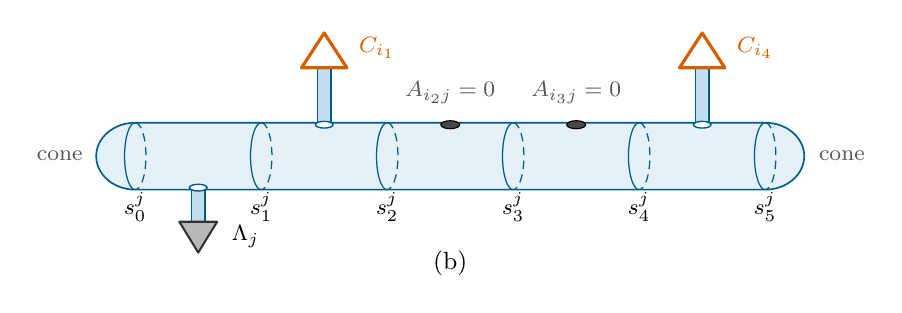
\begin{tikzpicture}[x=0.8cm,y=0.85cm,baseline=(pb.base)]
  %%% (c) one column surface: cone, tether socket, one socket per admissible position, cone
  \draw[gtube] (1.6,0.42) -- (1.6,-0.98);
  \draw[gtube] (3.6,0.42) -- (3.6,1.32);
  \draw[gtube] (9.6,0.42) -- (9.6,1.32);
  \draw[gsurf] (0.6,0.5) -- (10.6,0.5) arc (90:-90:0.62 and 0.5) -- (0.6,-0.5) arc (270:90:0.62 and 0.5) -- cycle;
  \foreach \x/\t in {0.6/0,2.6/1,4.6/2,6.6/3,8.6/4,10.6/5} {
    \draw[gLine,densely dashed,line width=0.45pt] (\x,0.5) arc (90:-90:0.17 and 0.5);
    \draw[gLine,line width=0.45pt] (\x,0.5) arc (90:270:0.17 and 0.5);
    \node[gsmall] at (\x,-0.76) {$s^j_{\t}$};
  }
  \draw[ghole] (1.6,-0.47) ellipse (0.14 and 0.05);
  \draw[ghole] (3.6,0.47) ellipse (0.14 and 0.05);
  \draw[gseal] (5.6,0.47) ellipse (0.15 and 0.06);
  \draw[gseal] (7.6,0.47) ellipse (0.15 and 0.06);
  \draw[ghole] (9.6,0.47) ellipse (0.14 and 0.05);
  \draw[growcyc] (3.24,1.32) -- (3.96,1.32) -- (3.6,1.84) -- cycle; \node[gsmall,text=gRow,anchor=west] at (4.0,1.62) {$C_{i_1}$};
  \draw[growcyc] (9.24,1.32) -- (9.96,1.32) -- (9.6,1.84) -- cycle; \node[gsmall,text=gRow,anchor=west] at (10.0,1.62) {$C_{i_4}$};
  \draw[gteth] (1.3,-0.98) -- (1.9,-0.98) -- (1.6,-1.44) -- cycle; \node[gsmall,anchor=west] at (1.98,-1.2) {$\Lambda_j$};
  \node[gsmall,text=black!65,anchor=east] at (-0.08,0.0) {cone};
  \node[gsmall,text=black!65,anchor=west] at (11.3,0.0) {cone};
  \foreach \xm/\t in {5.6/{$A_{i_2j}=0$},7.6/{$A_{i_3j}=0$}} \node[gsmall,text=black!65] at (\xm,0.95) {\t};
  \node[gpanel] (pb) at (5.6,-1.6) {(b)};
\end{tikzpicture}
\caption{The pieces of the gadget (Definition~\ref{def:gadget}).
(a)~A socket: the punctured cylinder, that is, the cylinder $\mathrm{Cyl}(a,b)$ between the triangle cycles $a$ and~$b$, cut open along the edge $a_0b_0$ (dashed; the two copies are identified), with the triangle $h=a_0a_1b_0$ removed (hatched), and its two possible attachments.
The hole~$h$ is either sealed by the single triangle~$h$ or tubed to a row cycle~$C_i$ by the six triangles of $\mathrm{Cyl}(h,C_i)$, so flipping one entry of~$A$ costs $1+6=7$ triangle updates (Lemma~\ref{lem:locality}).
(b)~The surface $\Sigma_j$ formed by the triangles of column~$j$: from left to right, a cone, the socket tubed to the tether~$\Lambda_j$, one socket per admissible position of column~$j$ (here four, in rows $i_1<i_2<i_3<i_4$, with $A_{i_1j}=A_{i_4j}=1$ and $A_{i_2j}=A_{i_3j}=0$), and a cone, glued in a chain along the triangle cycles $s^j_0,\dots,s^j_5$.}
\label{fig:socket}
\end{figure}
